\documentclass{article}
\usepackage{subfig}
\usepackage{graphicx}
\usepackage{graphics}
\usepackage{multirow}
\newcounter{row}
\usepackage{authblk}



\makeatletter
\@addtoreset{subfigure}{row}
\makeatother


%PDF Info Is Required:
%\pdfinfo{
%	/Title (2018 Formatting Instructions for Authors Using LaTeX)
%	/Author (AAAI Press Staff)}
\setcounter{secnumdepth}{0}  
\title{Analysing network structures of conversations in an online suicide support forum}
\date{\vspace{-5ex}}
\author[1]{Sagar Joglekar}
\author[1,2]{Sumithra Velupillai}
\author[2,]{Rina Dutta}
\author[1]{Nishanth Sastry}
\affil[1]{King's College, Department of Informatics, London, UK}
\affil[2]{King’s College London, IoPPN, London, SE5 8AF, UK}
\begin{document}
\label{sec:Supplementary}

\maketitle


\renewcommand\Authands{ and }

\section{Supplementary material}
We performed motif census for all the 36 Anchored triadic motifs across all BL and FP datasets. Figure \ref{fig:Rare_motifs} exhibits the trends in anchored motif census, for the insignificantly expressed or equally prevalent motifs.


 \begin{figure}[!htb]
    \renewcommand{\thesubfigure}{\arabic{row}.\alph{subfigure}}%
 	\centering
    \setcounter{row}{1}%
 	\subfloat[]{
 		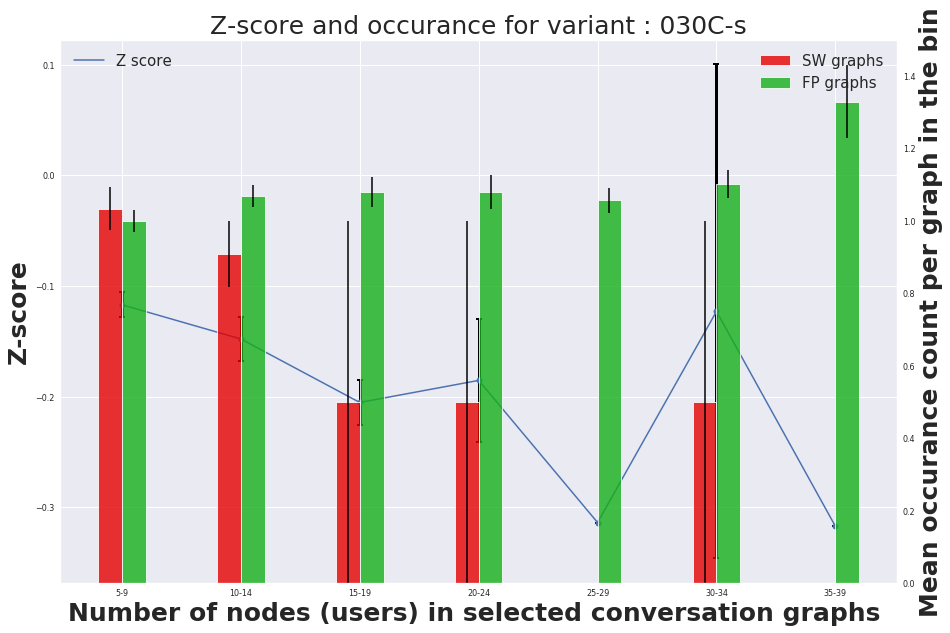
\includegraphics[width=0.3\textwidth]{Figures/Zscore/030C-a.png}
 	}
 	\subfloat[]{
 		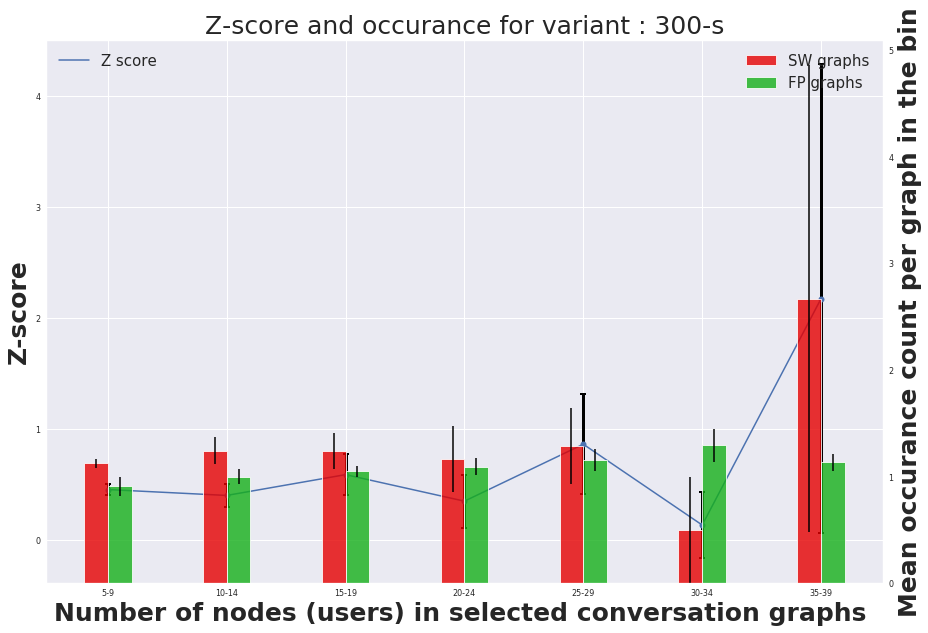
\includegraphics[width=0.3\textwidth ]{Figures/Zscore/300-s.png}
 	}
 	\subfloat[]{
 		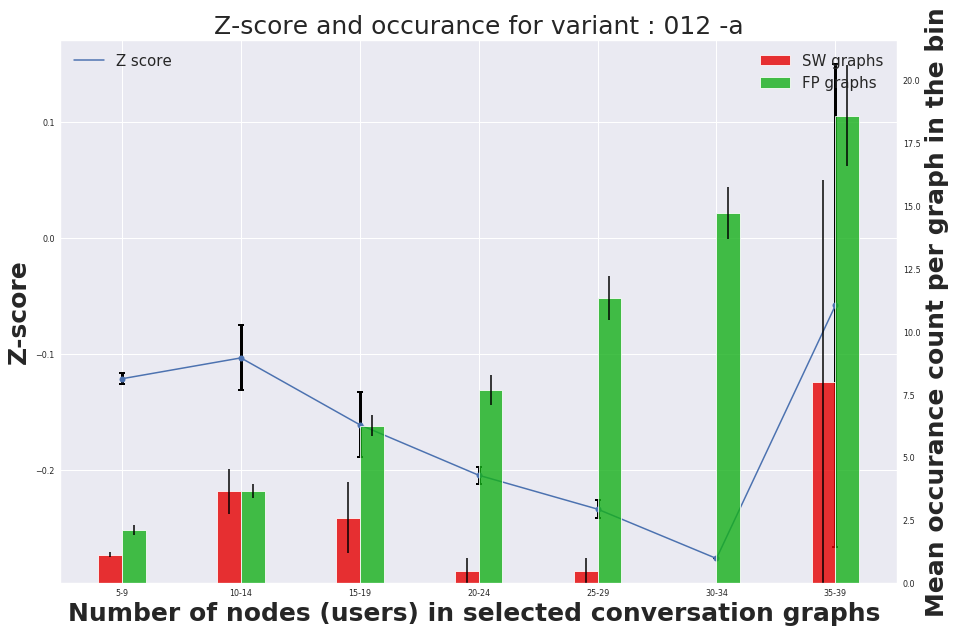
\includegraphics[width=0.3\textwidth]{Figures/Zscore/012-a.png}
 	}


    \stepcounter{row}%
 	\subfloat[]{
 	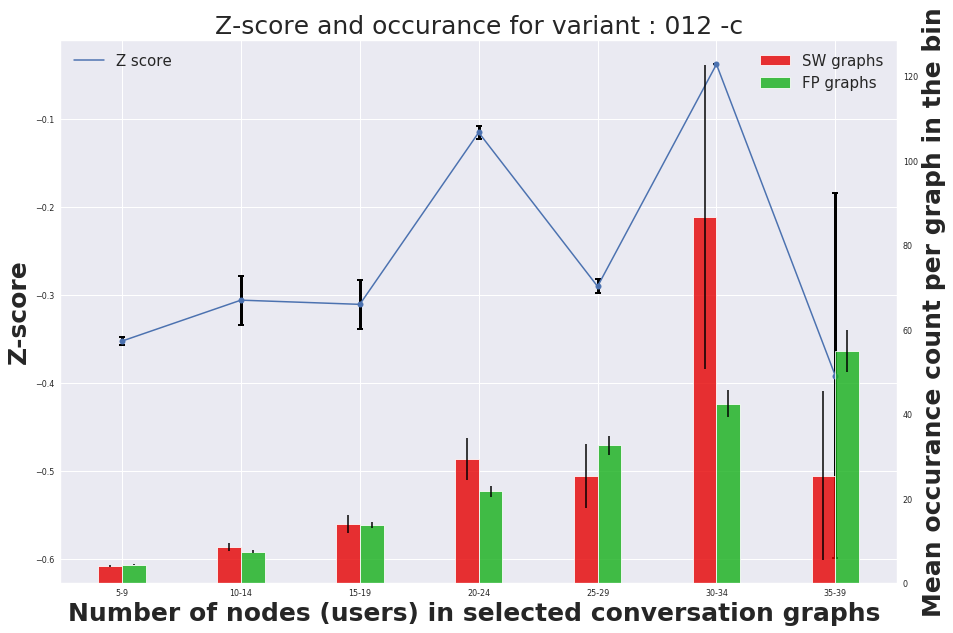
\includegraphics[width=0.3\textwidth ]{Figures/Zscore/012-c.png}
 	}
 	\subfloat[]{
 	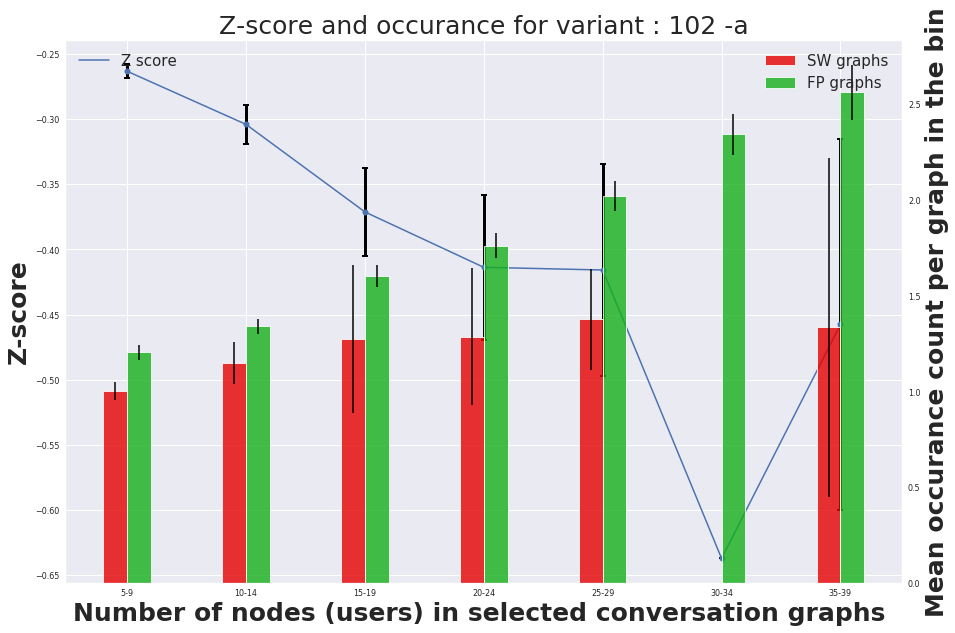
\includegraphics[width=0.3\textwidth]{Figures/Zscore/102-a.png}
 	}
    \subfloat[]{
 	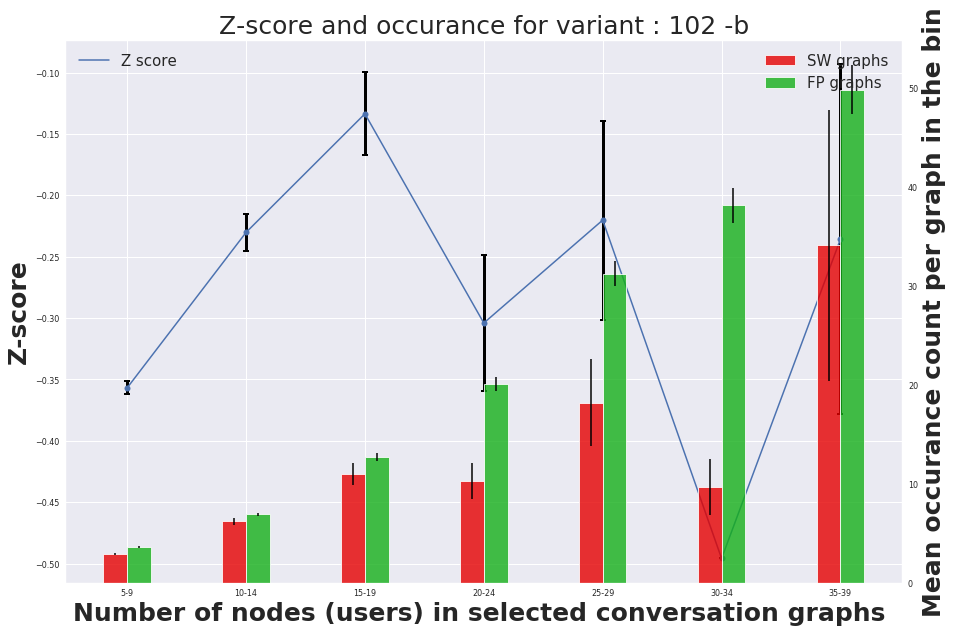
\includegraphics[width=0.3\textwidth]{Figures/Zscore/102-b.png}
 	}
	
    \stepcounter{row}%
    \subfloat[]{
 	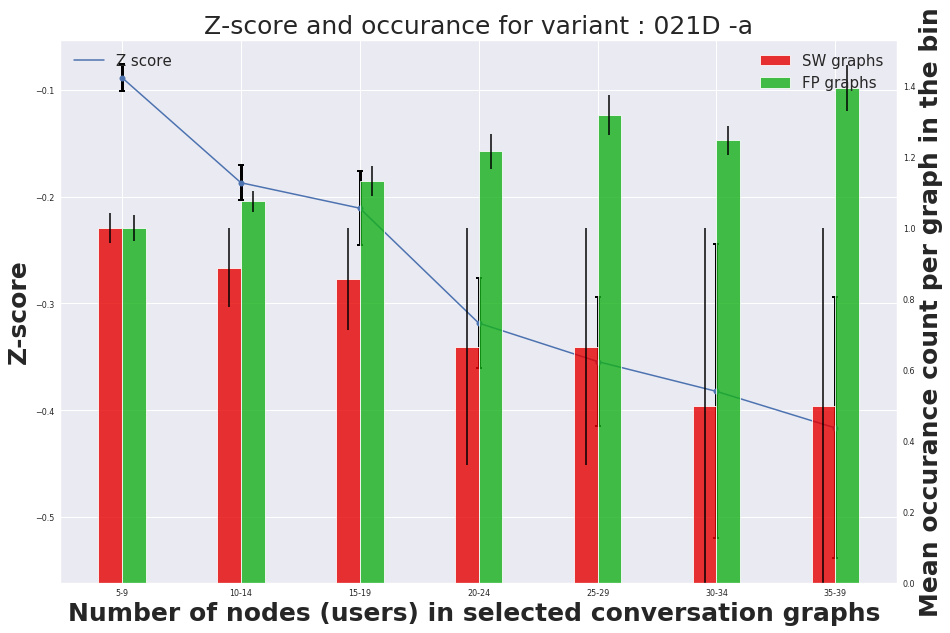
\includegraphics[width=0.3\textwidth ]{Figures/Zscore/021D-a.png}
 	}
 	\subfloat[]{
 	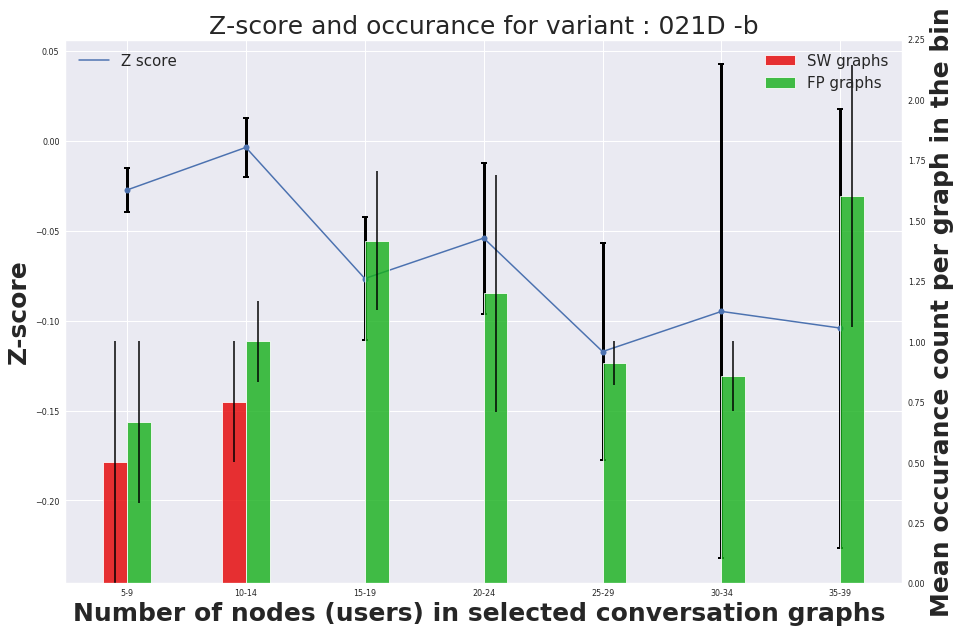
\includegraphics[width=0.3\textwidth ]{Figures/Zscore/021D-b.png}
 	}
    \subfloat[]{
 	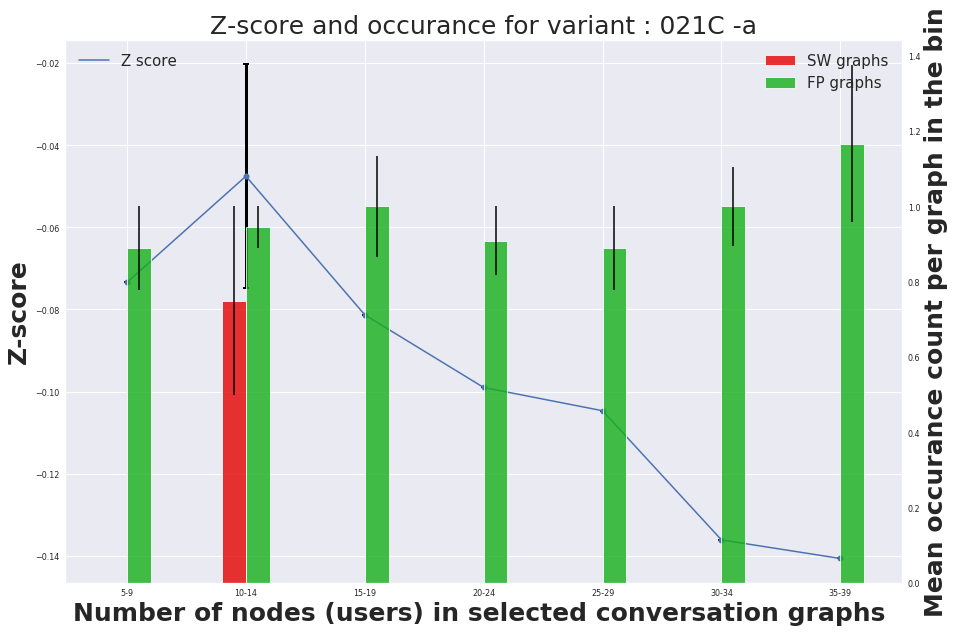
\includegraphics[width=0.3\textwidth]{Figures/Zscore/021C-a.png}
 	}
	
    
    \stepcounter{row}%
 	\subfloat[]{
 	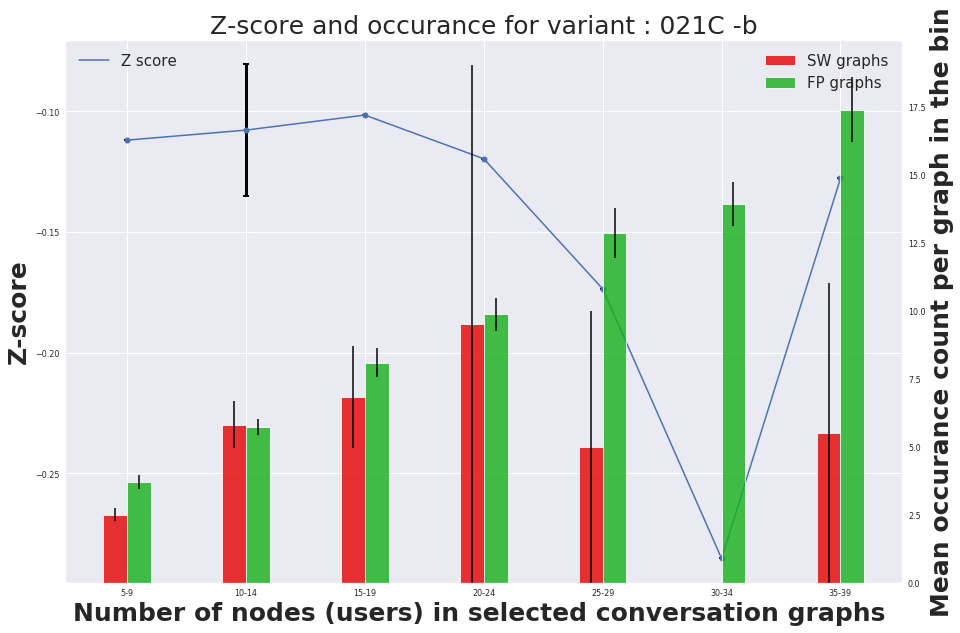
\includegraphics[width=0.3\textwidth]{Figures/Zscore/021C-b.png}
 	}
 	\subfloat[]{
 	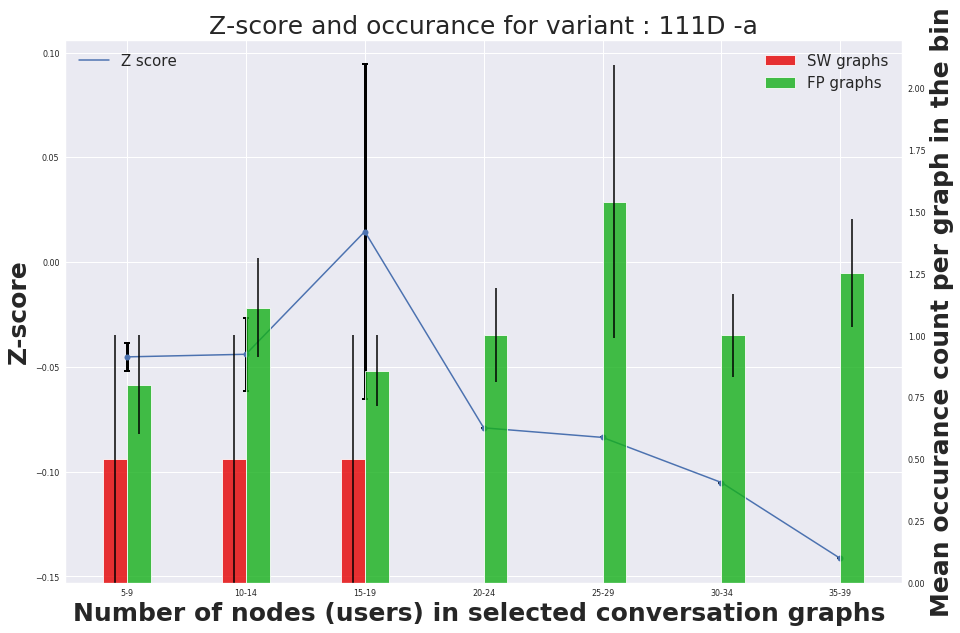
\includegraphics[width=0.3\textwidth ]{Figures/Zscore/111D-a.png}
 	}
 	\subfloat[]{
 	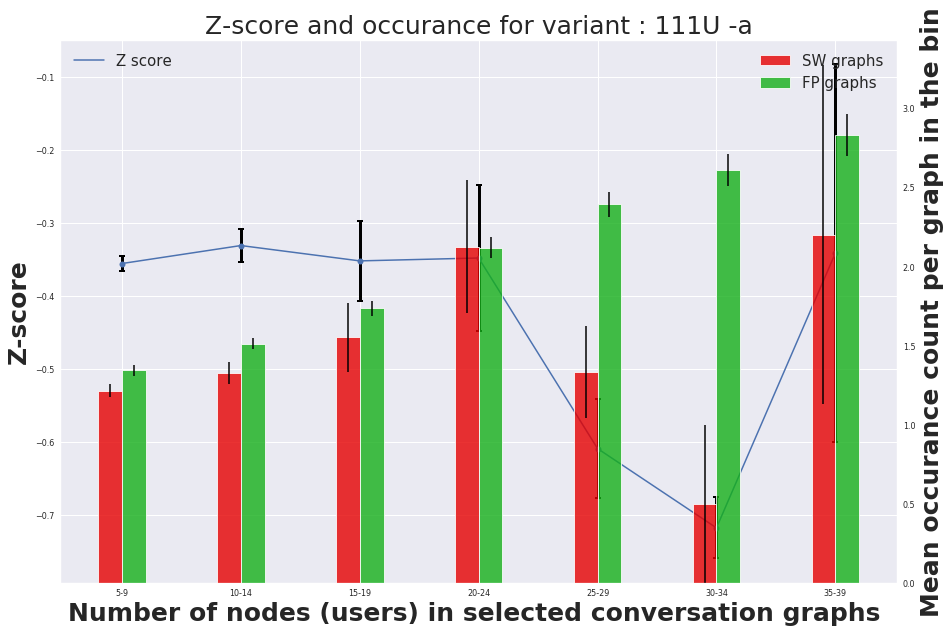
\includegraphics[width=0.3\textwidth ]{Figures/Zscore/111U-a.png}
 	}
    
    
    \stepcounter{row}%
   	\subfloat[]{
    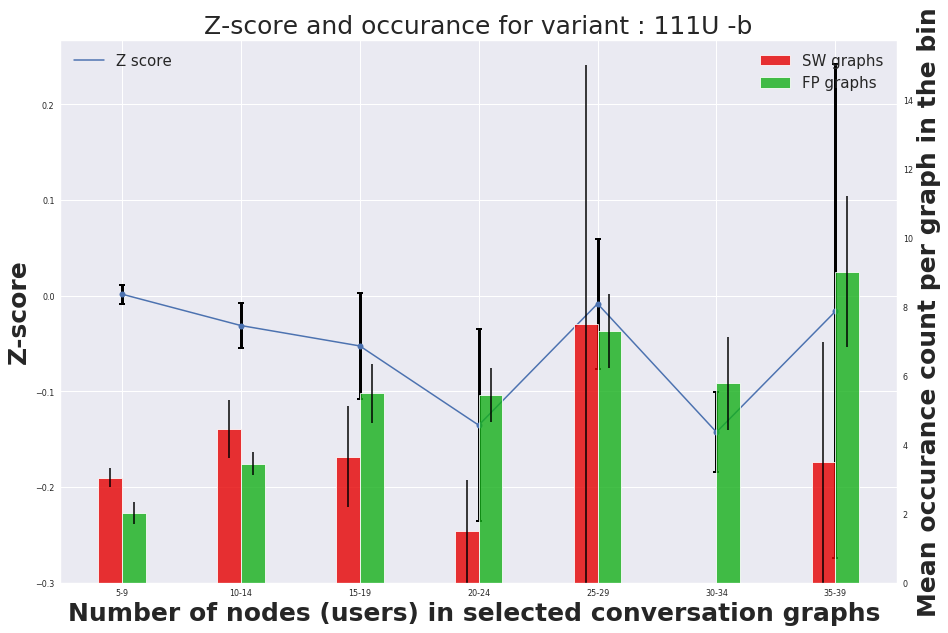
\includegraphics[width=0.3\textwidth]{Figures/Zscore/111U-b.png}
    }
    \subfloat[]{
    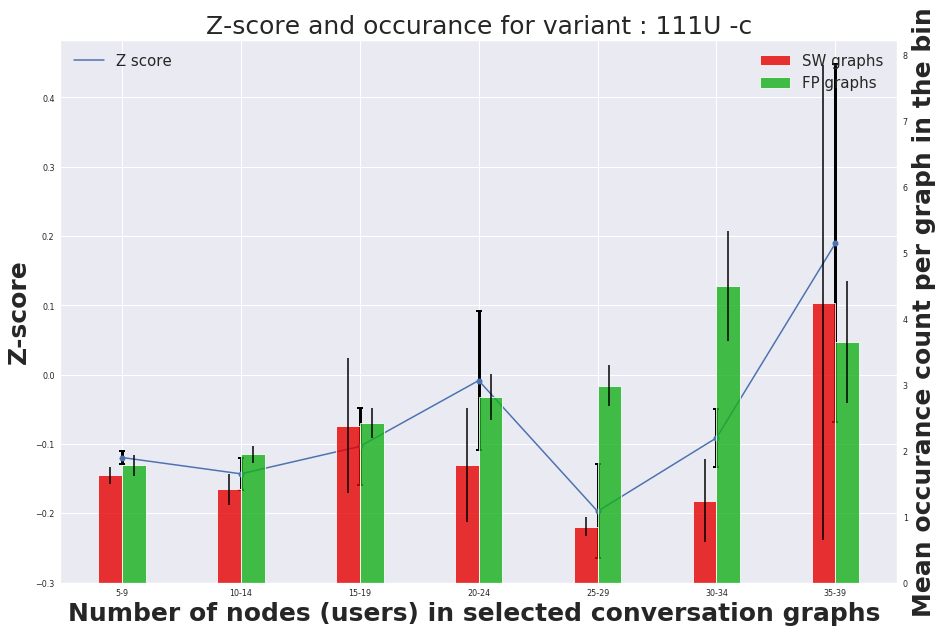
\includegraphics[width=0.3\textwidth ]{Figures/Zscore/111U-c.png}
    }
    \subfloat[]{
    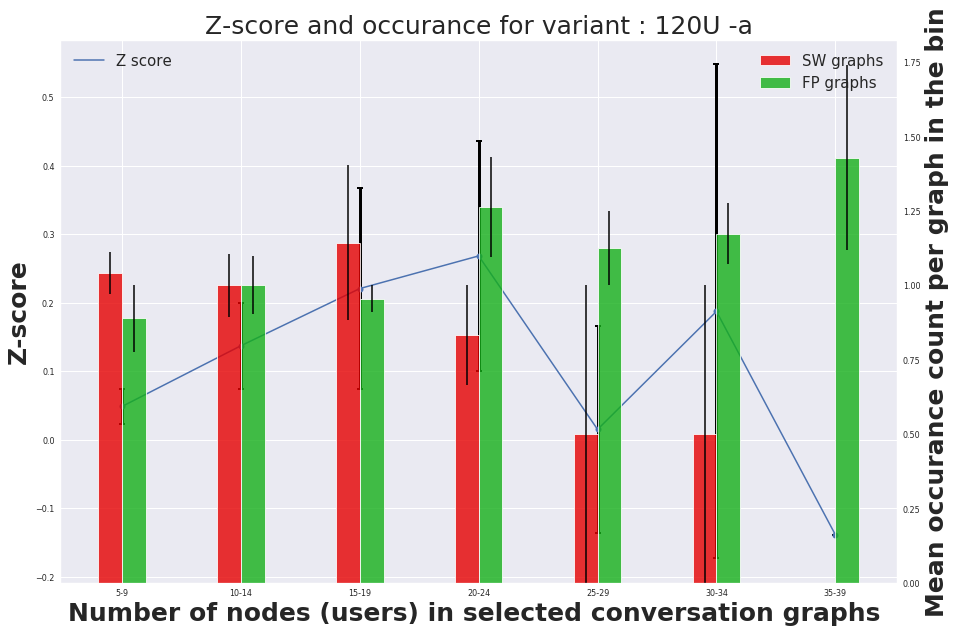
\includegraphics[width=0.3\textwidth]{Figures/Zscore/120U-a.png}
    }
 \end{figure}


 \begin{figure}[htb]\ContinuedFloat
    \renewcommand{\thesubfigure}{\arabic{row}.\alph{subfigure}}%
 	\centering
     
    \setcounter{row}{6}%
 	\subfloat[]{
 	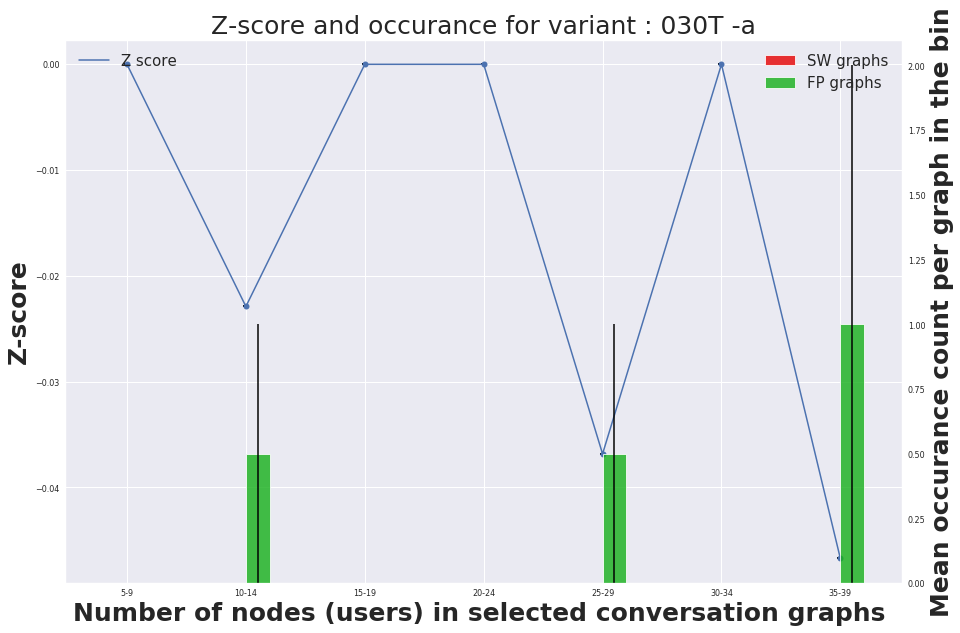
\includegraphics[width=0.3\textwidth]{Figures/Zscore/030T-a.png}
 	}
 	\subfloat[]{
 	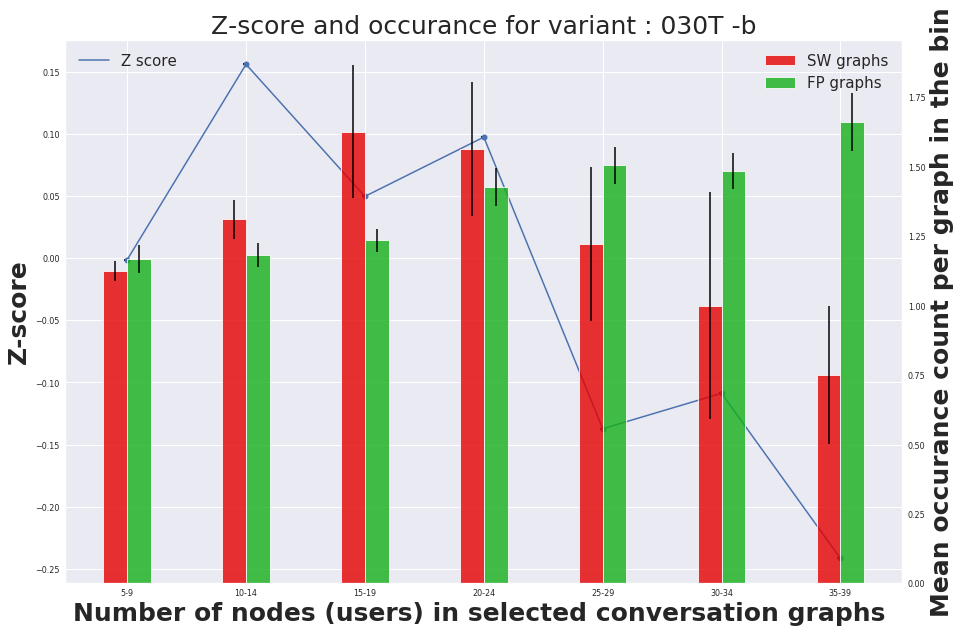
\includegraphics[width=0.3\textwidth ]{Figures/Zscore/030T-b.png}
 	}
 	\subfloat[]{
 	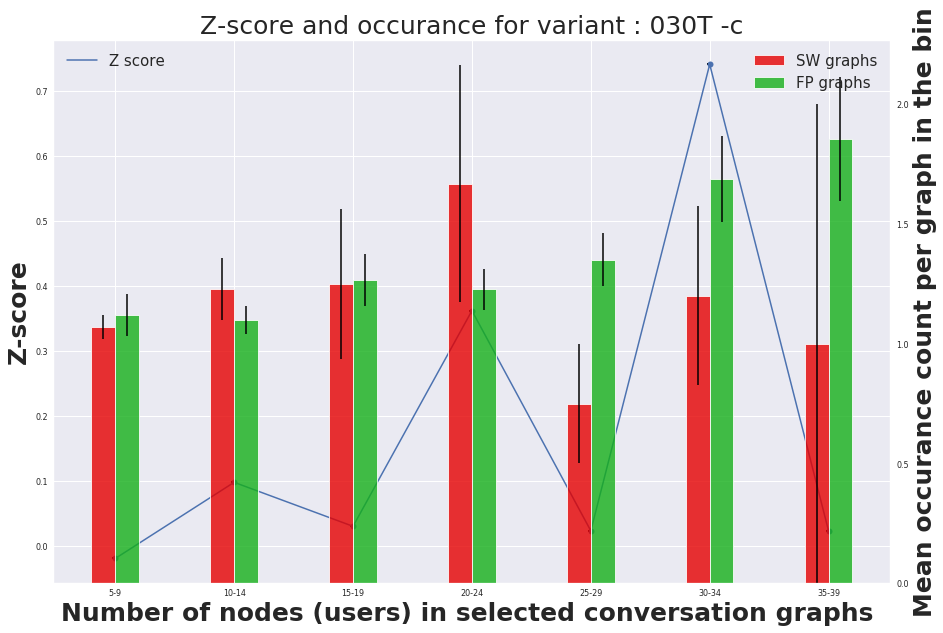
\includegraphics[width=0.3\textwidth]{Figures/Zscore/030T-c.png}
 	}
	
    \stepcounter{row}%
 	\subfloat[]{
 	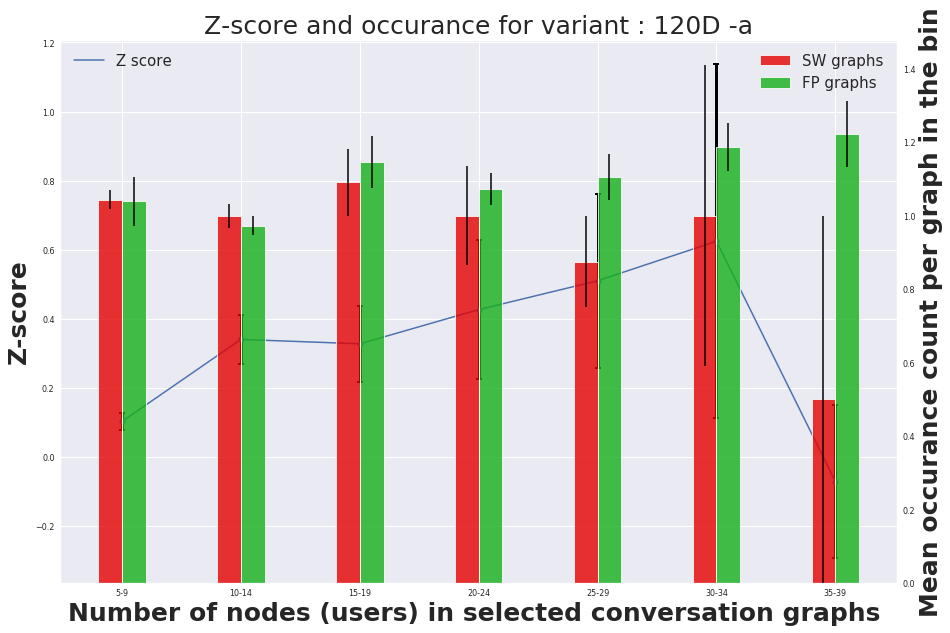
\includegraphics[width=0.3\textwidth]{Figures/Zscore/120D-a.png}
 	}
 	\subfloat[]{
 	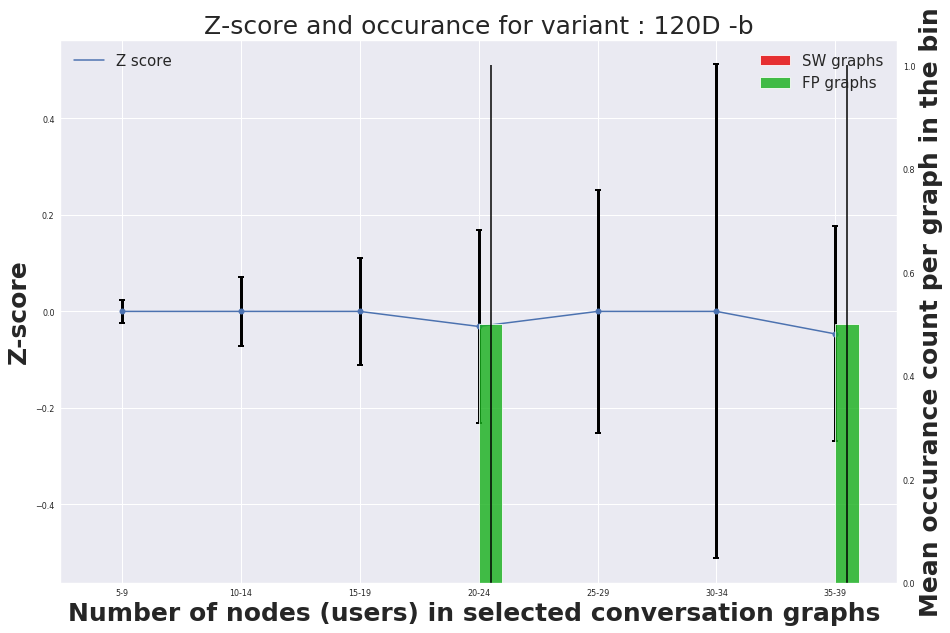
\includegraphics[width=0.3\textwidth ]{Figures/Zscore/120D-b.png}
 	}
 	\subfloat[]{
 	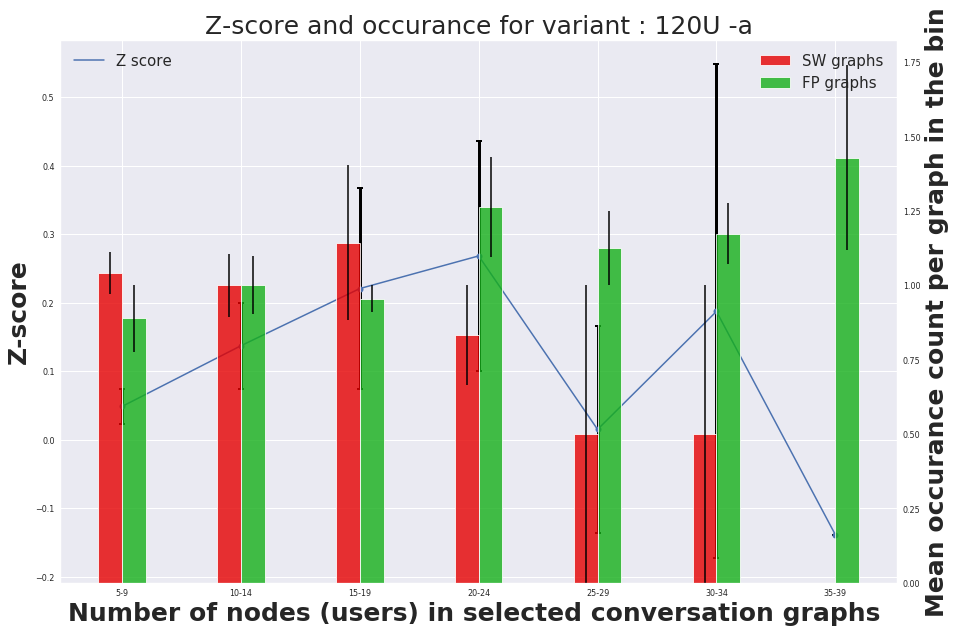
\includegraphics[width=0.3\textwidth ]{Figures/Zscore/120U-a.png}
 	}
	
    \stepcounter{row}%
    \subfloat[]{
    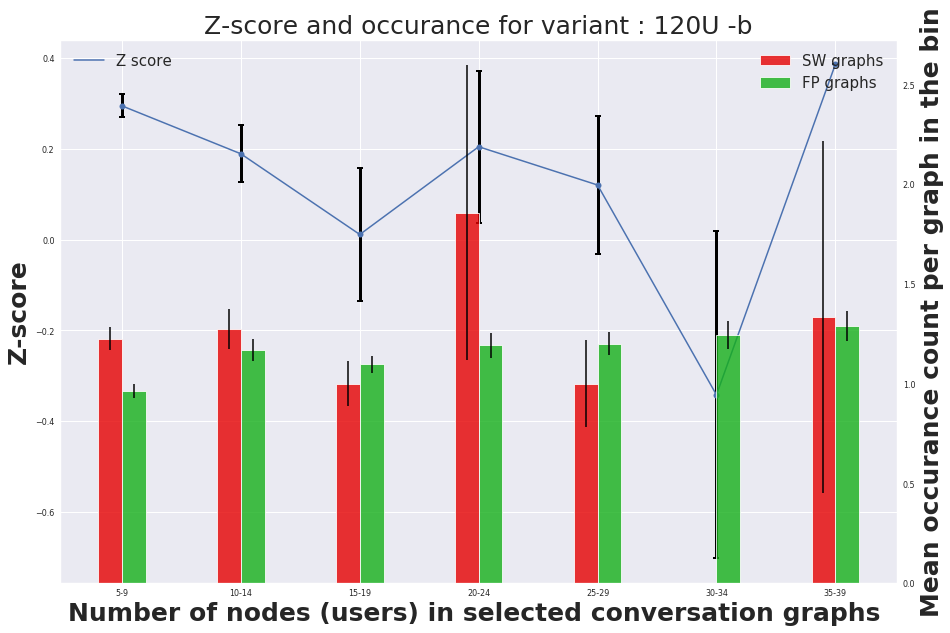
\includegraphics[width=0.3\textwidth ]{Figures/Zscore/120U-b.png}
    }
	\subfloat[]{
    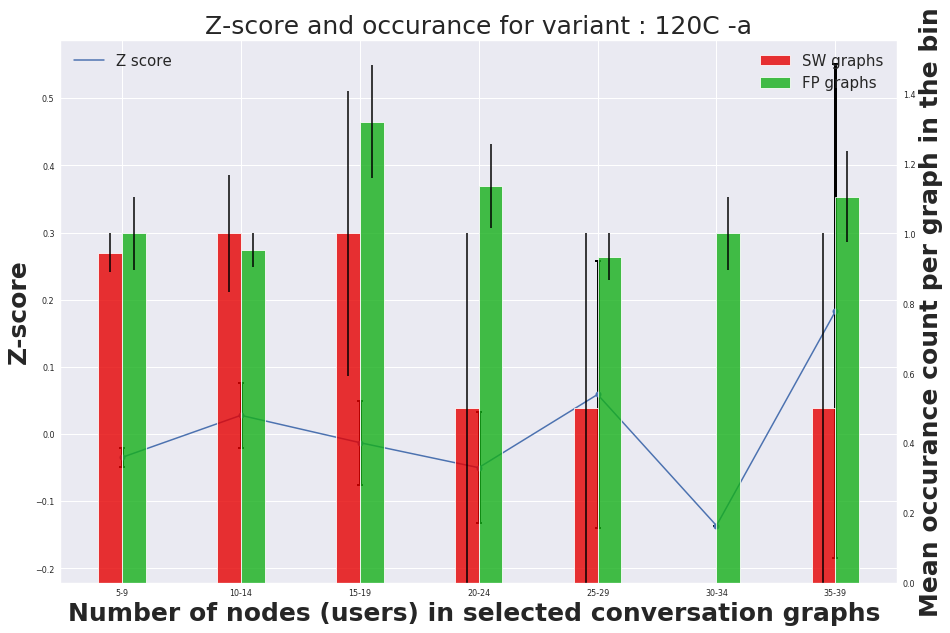
\includegraphics[width=0.3\linewidth ]{Figures/Zscore/120C-a.png}
    }
	\subfloat[]{
    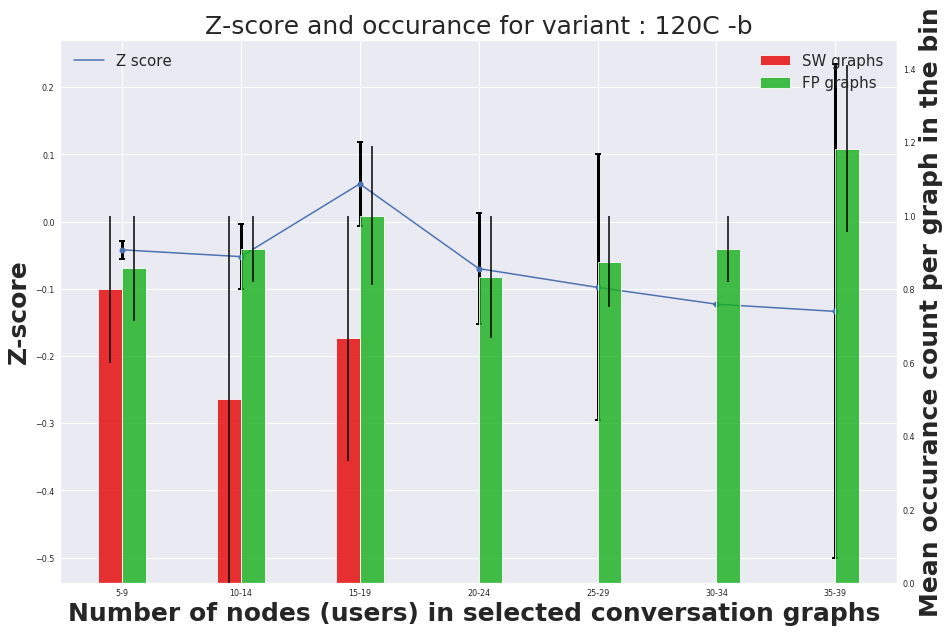
\includegraphics[width=0.3\linewidth ]{Figures/Zscore/120C-b.png}
    }


    \stepcounter{row}%
    \subfloat[]{
    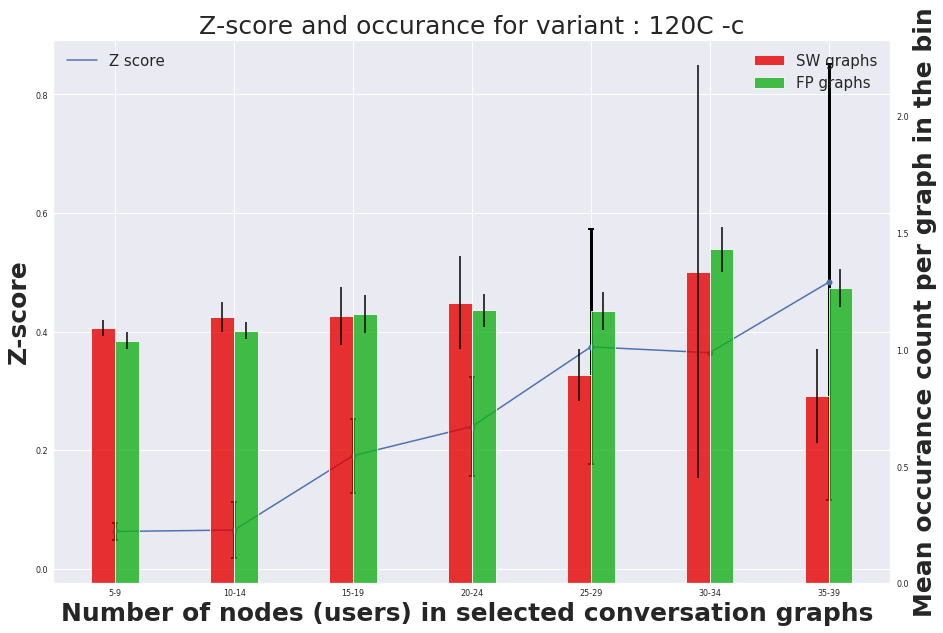
\includegraphics[width=0.3\textwidth ]{Figures/Zscore/120C-c.png}
    }
    \subfloat[]{
    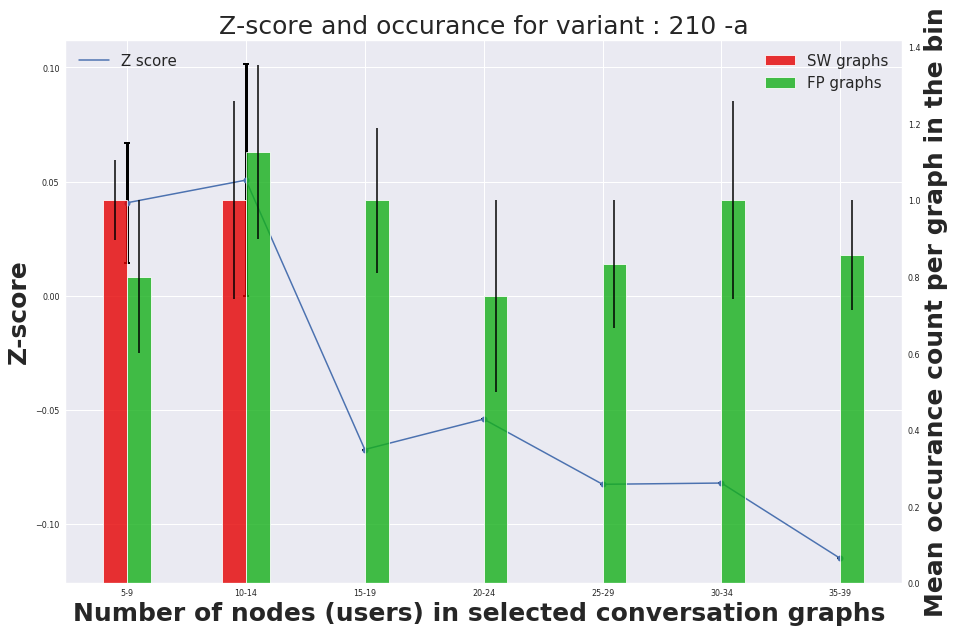
\includegraphics[width=0.3\linewidth ]{Figures/Zscore/210-a.png}
    }
    \subfloat[]{
    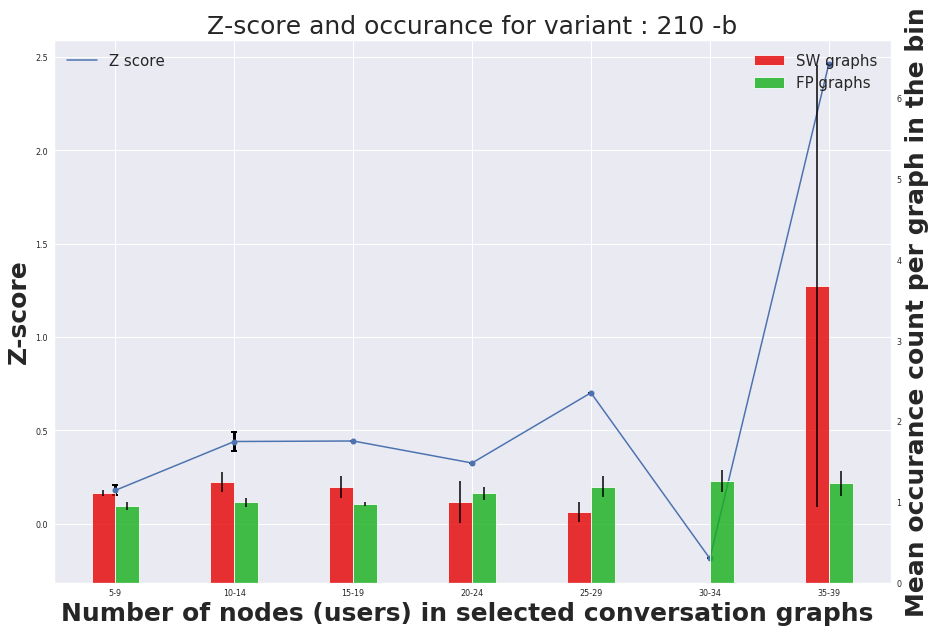
\includegraphics[width=0.3\linewidth ]{Figures/Zscore/210-b.png}
    }
    
    \stepcounter{row}%
    \subfloat[]{
    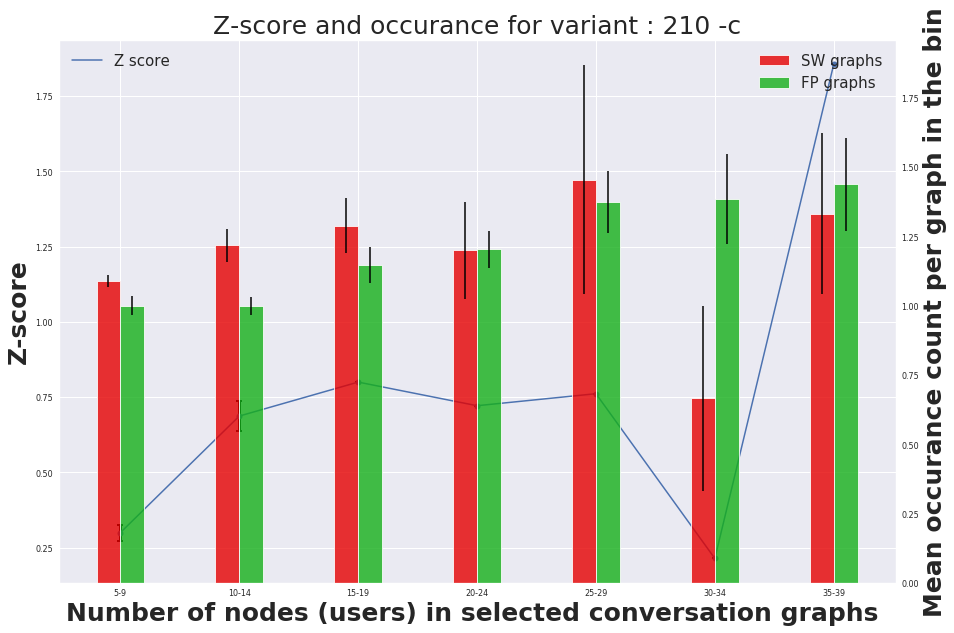
\includegraphics[width=0.3\linewidth ]{Figures/Zscore/210-c.png}
    }
 	\caption{ This figure lists all the insignificant Anchored motifs, either by the virtue of rare occurrence ($<$10 mean motifs per bin) or by account of low Z-score ($\left|Z\right|  < 1$).}
 	 \label{fig:Rare_motifs}
 \end{figure}

\end{document}